\chapter{Simulation de l'environnement}
\label{chapitre:environnement}
	
	\section{Introduction}

		La simulation de l'environnement est une partie importante du simulateur car c'est ce qui va définir le comportement des \gls{ROV}s dans leur milieu. Elle doit être très proche des conditions réelles afin d'avoir des résultats exploitables. Il faut donc établir les différents élements de l'environnements qui vont interagir avec les \gls{ROV}s afin de les intégrer dans le simulateur. Il y a principalement le milieu marin qui va ajouter une flottabilité au robots, mais aussi la présence de courants et enfin l'ombilical qui relie les \gls{ROV}s au bateau afin de l'alimenter en énergie mais aussi d'avoir un retour d'informations.

		La \textsc{Table}~\ref{table:elements} présente les différents élements qui peuvent être simulés dans un environnement marin.

		\begin{table}[ht]
			\centering
			\begin{tabular}{|c|c|}
				\hline
				Element & Simulation \\
				\hline
				Vent & \xmark\\
				\hline
				Vagues & \xmark\\
				\hline
				Courant sous-Marin & \cmark \\
				\hline
				Ombilical & \cmark \\
				\hline
			\end{tabular}
			\caption{Elements pris en compte dans l'environnement de simulation}
			\label{table:elements}
		\end{table}

	\section{Simulation d'environnements marins}

		

	\section{Simulation des courants marins}

		Une simulation des courants marins basée sur les équations de Navier-Stokes permet de proposer une approche intéressante à la simulation de courants marins~\cite{Garau2006current}.

	\section{Simulation d'ombilicaux}

		\subsection{Etat de l'art}

\subsection{Formalisme}

\subsection{Initialisation}
    L'initialisation des différents n\oe uds de l'ombilical est une étape importante car les coefficients du modèle comportemental sont reglés pour avoir un comportement cohérent lorsque la position du câble a convergée. Si l'initialisation est aléatoire, le temps du régime transitoire peut être long et la simulation peut ne pas être consistante.

    Pour initialiser l'ombilical, nous allons nous appuyer sur l'équation de la chaînette. Cette équation issue du calcul variationnel représente la forme que prend une corde attachée à ses deux extrémités afin de limiter son énergie. La \textsc{Figure}~\ref{fig:chainette} représente un tracé de cette équation.

    \begin{figure}[!htb]
        \centering
        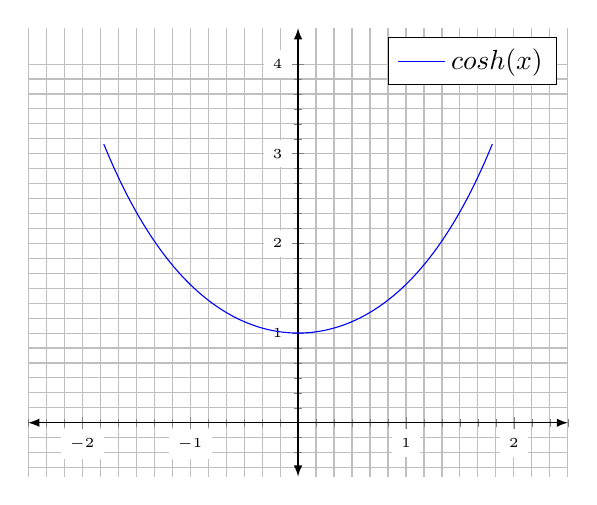
\begin{tikzpicture}
            \begin{axis}[
                    xmin=-2,   xmax=2,
                    ymin=-0.1,   ymax=3.9,
                    grid=both,
                    axis lines=middle,
                    minor tick num=5,
                    enlargelimits={abs=0.5},
                    axis line style={latex-latex},
                    ticklabel style={font=\tiny,fill=white},
                    xlabel style={at={(ticklabel* cs:1)},anchor=north west},
                    ylabel style={at={(ticklabel* cs:1)},anchor=south west}
                ]
                \addplot [
                    domain=-1.8:1.8, 
                    samples=100, 
                    color=blue,
                    ]
                    {cosh(\x)};
                \addlegendentry{$cosh(x)$}
            \end{axis}
        \end{tikzpicture}
        \caption{Représentation graphique de l'équation de la chaînette}
        \label{fig:chainette}
    \end{figure}
    

\subsection{Implémentation}
    L'implémentation d'un \gls{Plugin} \gls{Gazebo} permet de simuler le comportement de l'ombilical dans l'environnement de simulation. Ce \gls{Plugin} est basé sur l'instanciation d'objets de type \textit{Tether} et \textit{TetherElement}. L'objet \textit{Tether} possède les paramètres de simulation de l'ombilical, tandis que l'objet \textit{TetherElement} représente un tronçon de cet ombilical. Un diagramme de classe est présenté en \textsc{Figure}~\ref{fig:uml_class} et montre les différents attributs et méthodes associées à chaque classe.
    
    La \textit{Tether} utilise une structure de liste doublement chaînée\footnote{structure de données liée qui consiste en un ensemble n\oe uds liés les uns aux autres par des références au n\oe uds voisins.} de \textit{TetherElement}. Chaque \textit{TetherElement} possède alors une référence vers l'élément le précédant et l'élément le suivant, comme le montre la \textsc{Figure}~\label{fig:goubly_linked_list}. La \textit{Tether} ne possède ainsi qu'une référence vers le premier et le dernier n\oe ud de la chaîne, nommés respectivements \textit{head} et \textit{tail}. Il est ensuite possible de parcourir la chaîne de \textit{TetherElement} dans les deux sens en utilisant les références gardées par les \textit{TetherElement} eux-mêmes. 

    \begin{figure}[!htb]
        \centering
        \resizebox{0.90\textwidth}{!}{
            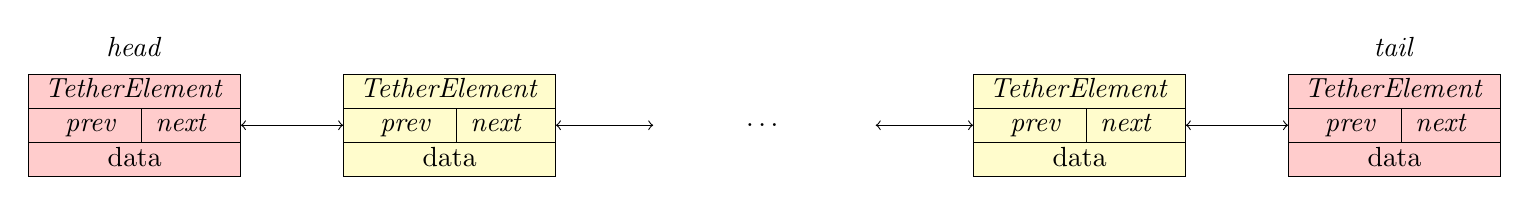
\begin{tikzpicture}
                \tikzset{TE/.style={draw, inner sep=0, outer sep=0, fill=yellow!20}}

                \node[TE, fill=red!20] (TE0) at (0,0) {\begin{tabular}{c} \textit{TetherElement} \\ \hline \hfill \textit{prev} \hfill \vline \hfill \textit{next} \hfill \\ \hline data \end{tabular}};

                \node[TE, fill=red!20] (TE4) at (16,0) {\begin{tabular}{c} \textit{TetherElement} \\ \hline \hfill \textit{prev} \hfill \vline \hfill \textit{next} \hfill \\ \hline data \end{tabular}};

                \foreach \i in {1,3} {
                    \node[TE] (TE\i) at (4*\i,0) {\begin{tabular}{c} \textit{TetherElement} \\ \hline \hfill \textit{prev} \hfill \vline \hfill \textit{next} \hfill \\ \hline data \end{tabular}};
                }
                \node[minimum width=80] (TE2) at (8,0) {\dots};
                \foreach \i in {0,1,2,3} {
                    \pgfmathtruncatemacro{\next}{\i +1}
                    \draw[<->] (TE\i) -- (TE\next);
                }

                \node (head) at (0,1) {\textit{head}};
                \node (tail) at (16,1) {\textit{tail}};
            \end{tikzpicture}
        }
        \caption{Liste doublement chainée}
        \label{fig:doubly_linked_list}
    \end{figure}

    \begin{figure}[!htb]
        \centering
        \resizebox{0.50\textwidth}{!}{
            \begin{tikzpicture}
                \begin{class}[text width=6cm]{Tether}{0,0}
                    \attribute{+ element\_mass : double}
                    \attribute{+ element\_volume : double}
                    \attribute{+ element\_length : double}
                    \attribute{+ position\_first : numpy.ndarray}
                    \attribute{+ position\_last : numpy.ndarray}
                    \attribute{+ elements : list of \textit{TetherElement}}
                \end{class}
            
                \begin{class}[text width=6cm]{TetherElement}{8.5,0}
                    \attribute{+ mass : double}
                    \attribute{+ volume : double}
                    \attribute{+ length : double}
                    \attribute{+ position : numpy.ndarray}
                    \attribute{+ velocity : numpy.ndarray}
                    \attribute{+ acceleration : numpy.ndarray}
                    \attribute{+ previous : TetherElement}
                    \attribute{+ next : TetherElement}
                    \attribute{+ K\_p : double}
                    \attribute{+ K\_d : double}
                    \attribute{+ K\_i : double}
                    \operation{+ F\_p(self) : numpy.ndarray}
                    \operation{+ F\_b(self) : numpy.ndarray}
                    \operation{+ F\_f(self) : numpy.ndarray}
                    \operation{+ Ft\_prev(self) : numpy.ndarray}
                    \operation{+ Ft\_next(self) : numpy.ndarray}
                \end{class}
            
                \aggregation{Tether}{}{~~~n}{TetherElement}
            \end{tikzpicture}
        }
        \caption{Diagramme de classe UML des classes \textit{Tether} et \textit{TetherElement}}
        \label{fig:uml_class}
    \end{figure}

\subsection{Suivi d'angles normalisés}
    Un problème avec la représentation numérique de l'orientation des solides est qu'elle est souvent normalisée, et les valeurs sont ainsi ramenées dans l'intervalle $[-\pi; \pi]$. On ne peut donc pas avoir l'orientation absolue, c'est à dire l'orientation d'un solide en prenant en compte les eventuels tours qu'il aurait pu faire sur lui-même.

    Pour résoudre ce problème, l'\textsc{Algorithme}~\ref{algo:suivi_angle} de suivi d'angles normalisés a été implémenté. Il prends en paramètres l'angle normalisé ainsi que l'angle précédemment calculé, et il retourne la valeur de l'angle absolu. L'idée de fournir l'angle précédent est de pouvoir retourner le nouvel angle qui se trouve dans le même quadrant et aussi de pouvoir suivre les sauts d'angles. Ainsi on peut suivre l'orientation absolue de solides en rotation dans l'espace, en ne fournissant que des orientations relatives ramenées dans l'intervalle $[-\pi; \pi]$, et en gardant en mémoire la précédente orientation calculée.
    
    \begin{algorithm}[!htb]
        \SetKwInOut{Input}{Entrées}
        \SetKwInOut{Output}{Sorties}
        \Entree{$angle\_normalise$, $angle\_absolu$}
        \Sortie{$angle\_absolu$}
        \Deb{
            $offset \leftarrow (angle\_absolu - angle\_normalise + \pi ) \pmod{2\pi}$ \\
            $angle\_absolu \leftarrow angle\_normalise + 2\pi \cdot offset$ \\
        }
        \Retour{$angle\_absolu$}

        \caption{Suivi d'angle} 
        \label{algo:suivi_angle}
    \end{algorithm}

    La \textsc{Figure}~\ref{fig:suivi_angle} présente les résultats de l'\textsc{Algorithme}~\ref{algo:suivi_angle} avec une angle variant dans l'intervalle $[-3\pi; 3\pi]$. On voit sur la première sous-figure l'angle réel et l'angle ramené dans l'intervalle $[-\pi; \pi]$ avec la présence de saut d'angles. Avec cette méthode, on est capable de suivre l'évolution de l'angle et de supprimer cess sauts afin de retrouver l'angle absolu visible dans la deuxième sous-figure et calculé uniquement à partir de la connaissance de l'angle normalisé.

    \begin{figure}[!htb]
        \centering
        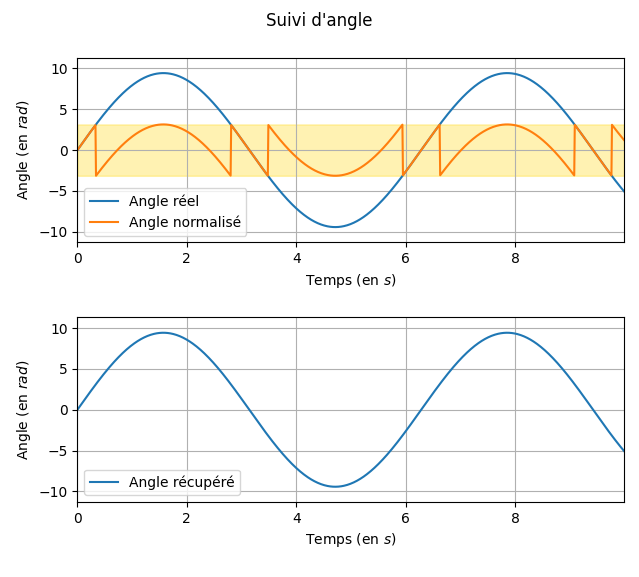
\includegraphics[width=0.5\textwidth]{suivi_angle.png}
        \caption{Suivi d'angle}
        \label{fig:suivi_angle}
    \end{figure}


\subsection{Resultats}
	